\documentclass{extbook}[14pt]
\usepackage{multicol, enumerate, enumitem, hyperref, color, soul, setspace, parskip, fancyhdr, amssymb, amsthm, amsmath, bbm, latexsym, units, mathtools}
\everymath{\displaystyle}
\usepackage[headsep=0.5cm,headheight=0cm, left=1 in,right= 1 in,top= 1 in,bottom= 1 in]{geometry}
\pagestyle{fancy}
\lhead{}
\chead{Answer Key for Module\,6\,-\,Polynomial\,Functions Version B}
\rhead{}
\lfoot{Summer\,C\,2020}
\cfoot{}
\rfoot{}
\begin{document}
\textbf{This key should allow you to understand why you choose the option you did (beyond just getting a question right or wrong). \href{https://xronos.clas.ufl.edu/mac1105spring2020/courseDescriptionAndMisc/Exams/LearningFromResults}{More instructions on how to use this key can be found here}.}

\textbf{If you have a suggestion to make the keys better, \href{https://forms.gle/CZkbZmPbC9XALEE88}{please fill out the short survey here}.}

\textit{Note: This key is auto-generated and may contain issues and/or errors. The keys are reviewed after each exam to ensure grading is done accurately. If there are issues (like duplicate options), they are noted in the offline gradebook. The keys are a work-in-progress to give students as many resources to improve as possible.}

\rule{\textwidth}{0.4pt}

26. Describe the zero behavior of the zero $x = -8$ of the polynomial below.
\[ f(x) = 7(x - 5)^{7}(x + 5)^{5}(x + 8)^{14}(x - 8)^{9} \] 

 
 The solution is  
 \begin{center} 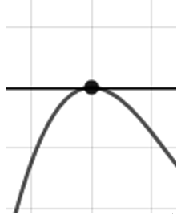
\includegraphics[width=0.3\textwidth]{../Figures/polyZeroBehaviorBB.png} \end{center}\begin{tabular}{|c|c|} 
\hline 
 & \tabularnewline 
 \textbf{A.} 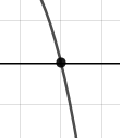
\includegraphics[width=0.3\textwidth]{../Figures/polyZeroBehaviorAB.png} & \textbf{B.} 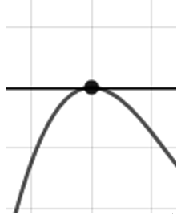
\includegraphics[width=0.3\textwidth]{../Figures/polyZeroBehaviorBB.png} \tabularnewline 
\hline 
 & \tabularnewline 
 \textbf{C.} 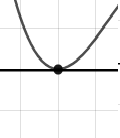
\includegraphics[width=0.3\textwidth]{../Figures/polyZeroBehaviorCB.png} & \textbf{D.} 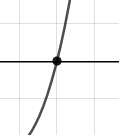
\includegraphics[width=0.3\textwidth]{../Figures/polyZeroBehaviorDB.png} \tabularnewline 
\hline 
 E. None of the figures above. & \tabularnewline 
\hline 
 \end{tabular} 
 
\begin{enumerate}[label=\Alph*.] 
\item   
\item   
\item   
\item   
\end{enumerate} 
 
\textbf{General Comments:} You will need to sketch the entire graph, then zoom in on the zero the question asks about.

-----------------------------------------------

27. Which of the following equations \textit{could} be of the graph presented below?
\begin{center} 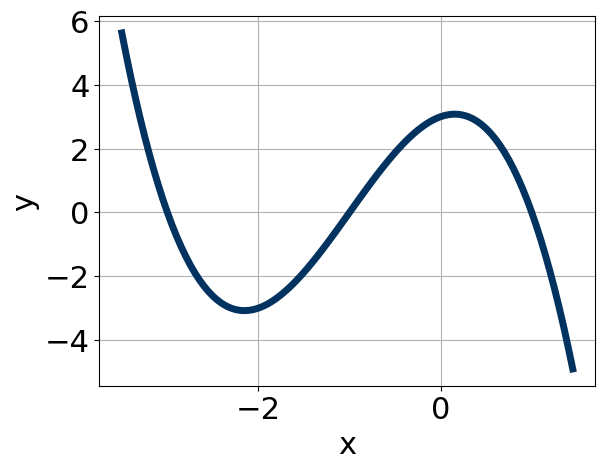
\includegraphics[width=0.3\textwidth]{../Figures/polyGraphToFunctionB.png} \end{center} 

The solution is $ 14(x + 1)^{5} (x - 1)^{5} (x + 2)^{5} $ 

\begin{enumerate}[label=\Alph*.] 
\item $ -2(x + 1)^{9} (x - 1)^{9} (x + 2)^{5} $ 

 This corresponds to the leading coefficient being the opposite value than it should be. 
\item $ 10(x + 1)^{10} (x - 1)^{4} (x + 2)^{5} $ 

 The factors $-1$ and $1$ have have been odd power. 
\item $ 15(x + 1)^{10} (x - 1)^{7} (x + 2)^{5} $ 

 The factor $-1$ should have been an odd power. 
\item $ -8(x + 1)^{10} (x - 1)^{11} (x + 2)^{9} $ 

 The factor $(x + 1)$ should have an odd power and the leading coefficient should be the opposite sign. 
\item $ 14(x + 1)^{5} (x - 1)^{5} (x + 2)^{5} $ 

 * This is the correct option. 
\end{enumerate} 
 
General Comments: Draw the x-axis to determine which zeros are touching (and so have even multiplicity) or cross (and have odd multiplicity).

-----------------------------------------------

28. Describe the end behavior of the polynomial below.
\[ f(x) = -9(x - 8)^{2}(x + 8)^{7}(x - 5)^{2}(x + 5)^{2} \] 

 
 The solution is  
 \begin{center} 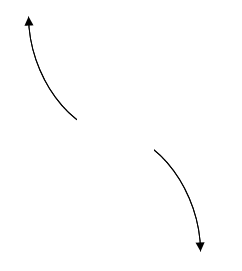
\includegraphics[width=0.3\textwidth]{../Figures/polyEndBehaviorAB.png} \end{center}\begin{tabular}{|c|c|} 
\hline 
 & \tabularnewline 
 \textbf{A.} 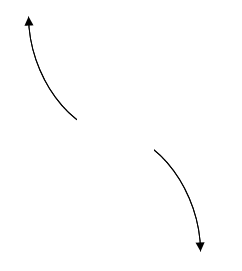
\includegraphics[width=0.3\textwidth]{../Figures/polyEndBehaviorAB.png} & \textbf{B.} 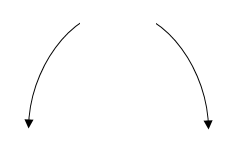
\includegraphics[width=0.3\textwidth]{../Figures/polyEndBehaviorBB.png} \tabularnewline 
\hline 
 & \tabularnewline 
 \textbf{C.} 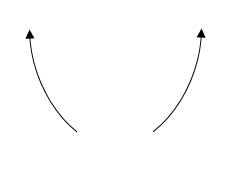
\includegraphics[width=0.3\textwidth]{../Figures/polyEndBehaviorCB.png} & \textbf{D.} 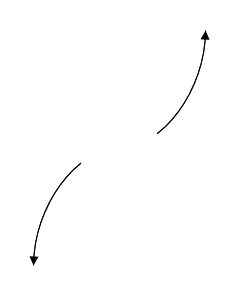
\includegraphics[width=0.3\textwidth]{../Figures/polyEndBehaviorDB.png} \tabularnewline 
\hline 
 E. None of the figures above. & \tabularnewline 
\hline 
 \end{tabular} 
 
\begin{enumerate}[label=\Alph*.] 
\item The function is above the $x$-axis, then passes through.  
\item The function is below the $x$-axis, then touches.  
\item The function is above the $x$-axis, then touches.  
\item The function is below the $x$-axis, then passes through.  
\end{enumerate} 
 
\textbf{General Comments:} Remember that end behavior is determined by the leading coefficient AND whether the \textbf{sum} of the multiplicities is positive or negative.

-----------------------------------------------

29. Construct the lowest-degree polynomial given the zeros below. Then, choose the intervals that contain the coefficients of the polynomial in the form $ax^3+bx^2+cx+d$.
\[ 3, \frac{7}{4}, \text{ and } \frac{-3}{2} \] 
The solution is $ 8x^{3} -26 x^{2} -15 x + 63 $ 

\begin{enumerate}[label=\Alph*.] 
\item $ a \in [-2, 10], b \in [24, 30], c \in [-21, -7], \text{ and } d \in [-69, -61] $ 

 $8x^{3} +26 x^{2} -15 x -63$, which corresponds to multiplying out $(x + 3)(4x + 7)(2x -3)$. 
\item $ a \in [-2, 10], b \in [37, 52], c \in [94, 102], \text{ and } d \in [62, 64] $ 

 $8x^{3} +50 x^{2} +99 x + 63$, which corresponds to multiplying out $(x + 1)(4x + 4)(2x -2)$. 
\item $ a \in [-2, 10], b \in [21, 24], c \in [-28, -25], \text{ and } d \in [-69, -61] $ 

 $8x^{3} +22 x^{2} -27 x -63$, which corresponds to multiplying out $(x + 1)(4x -4)(2x -2)$. 
\item $ a \in [-2, 10], b \in [-31, -20], c \in [-21, -7], \text{ and } d \in [-69, -61] $ 

 $8x^{3} -26 x^{2} -15 x -63$, which corresponds to multiplying everything correctly except the constant term. 
\item $ a \in [-2, 10], b \in [-31, -20], c \in [-21, -7], \text{ and } d \in [62, 64] $ 

 * $8x^{3} -26 x^{2} -15 x + 63$, which is the correct option. 
\end{enumerate} 
 
General Comments: To construct the lowest-degree polynomial, you want to multiply out $(x -3)(4x -7)(2x + 3)$

-----------------------------------------------

30. Construct the lowest-degree polynomial given the zeros below. Then, choose the intervals that contain the coefficients of the polynomial in the form $x^3+bx^2+cx+d$.
\[ -3 + 4i \text{ and } -1 \] 
The solution is $ x^{3} +7 x^{2} +31 x + 25 $ 

\begin{enumerate}[label=\Alph*.] 
\item $ b \in [5, 13], c \in [26, 32], \text{ and } d \in [18, 31] $ 

 * $x^{3} +7 x^{2} +31 x + 25$, which is the correct option. 
\item $ b \in [-1, 4], c \in [-9, -2], \text{ and } d \in [-7, 0] $ 

 $x^{3} + x^{2} -3 x -4$, which corresponds to multiplying out $(x -4)(x + 1)$. 
\item $ b \in [-9, -5], c \in [26, 32], \text{ and } d \in [-33, -20] $ 

 $x^{3} -7 x^{2} +31 x -25$, which corresponds to multiplying out $(x-(-3 + 4i))(x-(-3 - 4i))(x -1)$. 
\item $ b \in [-1, 4], c \in [1, 9], \text{ and } d \in [-1, 6] $ 

 $x^{3} + x^{2} +4 x + 3$, which corresponds to multiplying out $(x + 3)(x + 1)$. 
\item $ \text{None of the above.} $ 

 This corresponds to making an unanticipated error or not understanding how to use nonreal complex numbers to create the lowest-degree polynomial. If you chose this and are not sure what you did wrong, please contact the coordinator for help. 
\end{enumerate} 
 
General Comments: Remember that the conjugate of $a+bi$ is $a-bi$. Since these zeros always come in pairs, we need to multiply out $(x-(-3 + 4i))(x-(-3 - 4i))(x-(-1))$.

-----------------------------------------------


\end{document}

